\documentclass{beamer}

\usepackage{listings}
\usepackage{color}
\usepackage{xcolor}
\usepackage{ulem}
\usepackage{tikz}
\usepackage{graphicx}
\usetikzlibrary{positioning, shapes.geometric}
\definecolor{green}{rgb}{0,0.6,0}
\definecolor{gray}{rgb}{0.5,0.5,0.5}
\definecolor{mauve}{rgb}{0.58,0,0.82}
% init

\usetheme{Madrid}
\setbeamertemplate{itemize items}[triangle]
\setbeamertemplate{enumerate items}[default]
\lstset{
    frame=none,
    language=Java,
    showstringspaces=false,
    columns=fullflexible,
    basicstyle = \ttfamily\small,
    numbers=none,
    numberstyle=\tiny\color{gray},
    keywordstyle=\color{blue},
    commentstyle=\color{green},
    stringstyle=\color{mauve},
    breaklines=true,
    morekeywords={String,in,out, cd},
    breakatwhitespace=true,
    tabsize=4
}
% appearance setup

\title{CS109 Lab 7} % title here
\author{Ben Chen}
\institute{SUSTech}
\date{\today}

\begin{document}
\frame{\titlepage}

\begin{frame}
    \frametitle{What is git?}
Git is a version control system that helps you,
\begin{itemize}
    \item track the changes of your source code.\newline
    \textit{e.g.} update your v1.0 program to v2.0
    \item cooperate with your team.\newline
    \textit{e.g.} sync with the progress of your team
    \item \sout{get bonus for your project.}\newline
    we think using git is a normal action for project
\end{itemize}
\end{frame}

\begin{frame}[fragile]
    \frametitle{Installation}
    You need to follow these steps to install git,
    \begin{itemize}
        \item For Mac users, try Xcode or Homebrew in Terminal\newline
        \lstinline|xcode-select --install| or \lstinline|brew install git|
        \item For Windows users, use git for Windows\newline
        download from \url{https://gitforwindows.org}
        \item For Linux/Unix users, you should already know how to install git since you're using *nix.
    \end{itemize}
\end{frame}

\begin{frame}[fragile]
    \frametitle{Create your repository}
Your project is stored in a repo, which is within a folder.
\begin{itemize}
    \item In your project folder, use this to create a repo.
    \begin{lstlisting}[morekeywords=git]
cd /path/to/your/project
git init
    \end{lstlisting}
    \item To download an existing repo, use
    \begin{lstlisting}[morekeywords=git]
git clone <url>
    \end{lstlisting}
\end{itemize}
\end{frame}

\begin{frame}[fragile]
    \frametitle{Saving changes}
    \begin{columns}
        \begin{column}{0.4\textwidth}
            \centering
            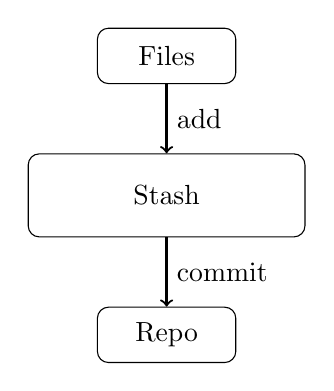
\begin{tikzpicture}[node distance=25pt]
                \node[draw, minimum width=50pt, minimum height=20pt, rounded corners](files){Files};
                \node[draw, minimum width=100pt, minimum height=30pt, rounded corners, below=of files](stash){Stash};
                \node[draw, minimum width=50pt, minimum height=20pt, rounded corners, below=of stash]      (repo)    {Repo};
                
                \draw[->, thick] (files)  -- node[right]{add}  (stash);
                \draw[->, thick] (stash)  -- node[right]{commit}  (repo);
              \end{tikzpicture}
        \end{column}
        \begin{column}{0.5\textwidth}
            To save changes, you should
            \begin{enumerate}
                \item add new or modified files to stash to pack them together
                \begin{lstlisting}[morekeywords=git]
git add Demo.java
git add Readme.md
                \end{lstlisting}
                \item commit the files in stash and write a comment
                \begin{lstlisting}[morekeywords=git]
git commit -m "add demo and readme doc"
                \end{lstlisting}
                \item remove files from stash and repo
                \begin{lstlisting}[morekeywords=git]
git remove <file>
                \end{lstlisting}
            \end{enumerate}
        \end{column}
    \end{columns}
\end{frame}

\begin{frame}[fragile]
    \frametitle{Check Something}
\begin{itemize}
    \item Check the status of stash
    \begin{lstlisting}[morekeywords=git]
git status
    \end{lstlisting}
    \item Check the history of the repo
    \begin{lstlisting}[morekeywords=git]
git log
    \end{lstlisting}
    \item Check the history of file
    \begin{lstlisting}[morekeywords=git]
git blame <file>
    \end{lstlisting}
\end{itemize}
\end{frame}

\begin{frame}[fragile]
    \frametitle{Version}
    \begin{columns}
        \begin{column}{0.5\textwidth}
            \centering
            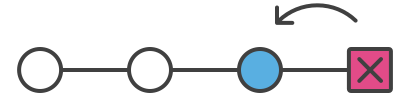
\includegraphics[width=0.8\textwidth]{hero.png}
        \end{column}
        \begin{column}{0.5\textwidth}
            To undo changes and go back to some version
            \begin{itemize}
                \item go back to last version
                \begin{lstlisting}[morekeywords=git]
git reset --hard HEAD^
                \end{lstlisting}
                \item go back to last 3 version
                \begin{lstlisting}[morekeywords=git]
git reset --hard HEAD~3
                \end{lstlisting}
                \item go back to specific version
                \begin{lstlisting}[morekeywords=git]
git reset --hard <id>
// commit id is at git log
                \end{lstlisting}
            \end{itemize}
        \end{column}
    \end{columns}
\end{frame}

\begin{frame}
    \frametitle{Remote Repo}
Generally, we use the website Github as our remote repo.
\begin{enumerate}
    \item Sign up in \url{https://github.com}
    \item Create a new blank repo
    \item Use \lstinline|git clone| to download the repo
    \item In Settings, add your teammates at Collaborators
    \item Start developing your project!
\end{enumerate}
\end{frame}

\begin{frame}[fragile]
    \frametitle{Remote Repo}
In local computer, we can use these commands,
\begin{itemize}
    \item To sync with your current progress
    \begin{lstlisting}[morekeywords=git]
git fetch origin // origin is alias of github address
    \end{lstlisting}
    \item To push your new version to remote
    \begin{lstlisting}[morekeywords=git]
git push origin main // main is the name of branch
    \end{lstlisting}
\end{itemize}
\end{frame}

\begin{frame}[fragile]
    \frametitle{Wildcard Character}
Wildcard is a symbol used to represent more characters
\begin{itemize}
    \item * is used to match any characters
    \begin{lstlisting}[morekeywords=git]
git add *.java // add any .java file
git add * // add all files
git add Demo.* // add any files named Demo
    \end{lstlisting}
    \item ? is used to match one character
    \begin{lstlisting}[morekeywords=git]
git add ???.java // add .java with name of 3 characters
    \end{lstlisting}
    \item More...
\end{itemize}
\end{frame}

\begin{frame}
    \frametitle{To be continued...}
You may look them up by yourself, 
\begin{itemize}
    \item Branch and Conflict Resolving
    \item \textit{.gitignore} file
    \item Lisence for your repo
    \item Git config
    \item You tell me
\end{itemize}
\end{frame}

\end{document}
